\documentclass{beamer}
\usepackage{polski}
\usepackage[utf8]{inputenc}
\usepackage{graphics}
\usepackage{minted}
\usepackage{fvextra}
\usepackage{caption}
\usepackage{epigraph}
\usepackage{array}
\usepackage{multimedia}
\newcolumntype{L}[1]{>{\raggedright\let\newline\\\arraybackslash\hspace{0pt}}m{#1}}
\newcolumntype{C}[1]{>{\centering\let\newline\\\arraybackslash\hspace{0pt}}m{#1}}
\newcolumntype{R}[1]{>{\raggedleft\let\newline\\\arraybackslash\hspace{0pt}}m{#1}}
\definecolor{NiceGreen}{RGB}{40,200,0}
\definecolor{CoolDarkGray}{RGB}{50,50,50}

\title{\texttt{Projekt aplikacji do ekstremalnego uczenia maszynowego do klasyfikacji big data}}
\author{Autorzy: Ahmed Abdelkarim, Aleksandra Hernik \\ Promotor: dr hab. inż. Jerzy Balicki, prof. PW}

\begin{document}
\setbeamercolor{background canvas}{bg=CoolDarkGray}
\setbeamercolor{title}{fg=NiceGreen}
\setbeamercolor{frametitle}{fg=NiceGreen}
\setbeamercolor{structure}{fg=white}
\setbeamertemplate{section in toc}{%
    \textcolor{NiceGreen}{\inserttocsectionnumber)}   \inserttocsection \par}

\addtobeamertemplate{navigation symbols}{}{%
    \usebeamerfont{footline}%
    \usebeamercolor[fg]{footline}%
    \hspace{1em}%
    \insertframenumber/\inserttotalframenumber
}

\setbeamercolor{normal text}{fg=white}\usebeamercolor*{normal text}
\begin{frame}
\begin{table}[H]
\begin{tabular}{p{\textwidth - 25mm + \oddsidemargin} l}
  
\includegraphics[width=25mm, height=25mm]{MiNI.png} &  
\includegraphics[width=25mm, height=25mm]{PW.png}
\end{tabular}
\end{table}


  \maketitle
\end{frame}

\begin{frame}{Plan}
  \tableofcontents[currentsection]
\end{frame}

\section{Wprowadzenie do ekstremalnego uczenia maszynowego}
\begin{frame}{Czym jest ekstremalne uczenie maszzynowe?}
\begin{figure}[H]
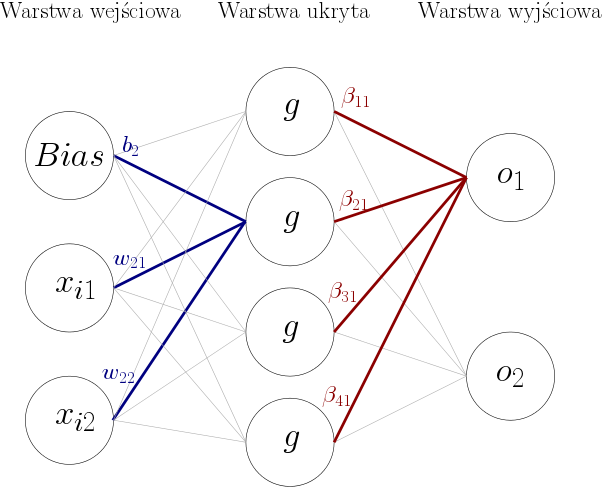
\includegraphics[scale=0.5]{schemat_sieci.png}
\caption{Sieć ELM}
\end{figure}
\end{frame}
\section{Cele}
\begin{frame}{Cele}
\begin{itemize}
\item Sprawdzenie wydajności i skuteczności metody
\item Stworzenie i porównanie dwóch aplikacji
\end{itemize}
\end{frame}
\section{Prezentacja aplikacji}

\section{Wyniki}
\begin{frame}{Benchmarki}

\begin{columns}
\begin{column}[T]{0.5\textwidth}
Klasyfikacja obszarów lasu ze względu na dominujące drzewa:

\begin{itemize}
\item 15 120 próbek
\item 54 kolumny, w tym 44~binarne
\item 7 możliwych klas:
\begin{itemize}
\item świerk/jodła,
\item sosna wydmowa,
\item sosna żółta,
\item topola/wierzba,
\item osika,
\item daglezja zielona,
\item \textit{krummholz}
\end{itemize}
\end{itemize}
\end{column}
\begin{column}[T]{0.5\textwidth}
Klasyfikacja meczów w grze Dota~2 ze względu na zwycięzcę:

\begin{itemize}
\item 50 000 próbek
\item 10 kolumn, w tym 6~nieistotnych
\item 2 możliwe klasy:
\begin{itemize}
\item zwycięstwo zespołu \textit{Radiant}
\item zwycięstwo zespołu \textit{Dire}
\end{itemize}
\end{itemize}
\end{column}
\end{columns}

\end{frame}

\begin{frame}{Skuteczność aplikacji w Pythonie}
\begin{figure}[H]
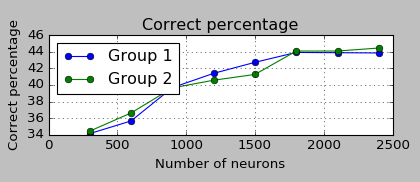
\includegraphics[width=\textwidth]{wyniki_forest_python_percentage.png}
\caption{Jakość uczenia}
\end{figure}
\end{frame}

\begin{frame}{Szybkość aplikacji w Pythonie}
\begin{figure}[H]
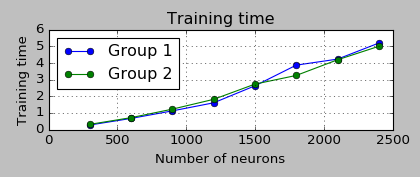
\includegraphics[width=\textwidth]{wyniki_forest_python_training_time.png}
\caption{Czas uczenia}
\end{figure}
\end{frame}

\begin{frame}{Skuteczność aplikacji w Matlabie}
\begin{figure}[H]
\centering
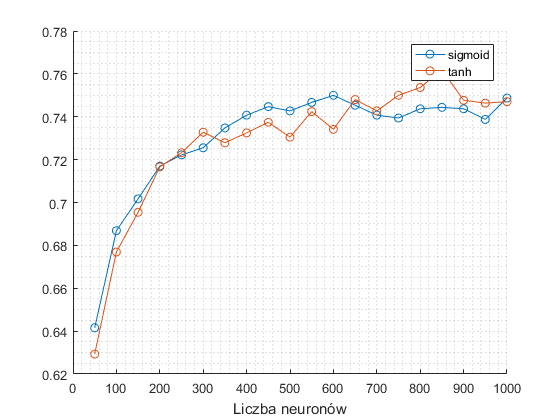
\includegraphics[width=0.85\textwidth]{forest_liczba_neuronow.png}
\caption{Jakość uczenia}
\end{figure}
\end{frame}

\begin{frame}{Szybkość aplikacji w Matlabie}
\begin{figure}[H]
\centering
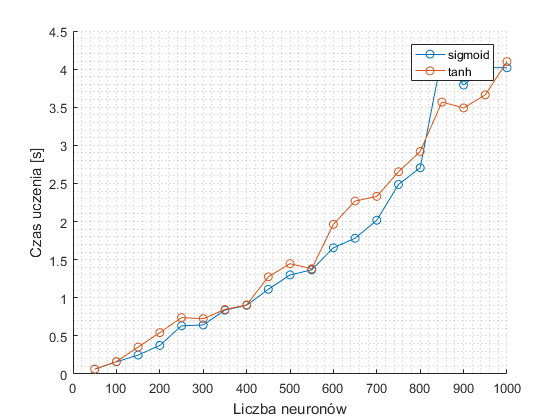
\includegraphics[width=0.85\textwidth]{forest_wydajnosc.png}
\caption{Czas uczenia}
\end{figure}
\end{frame}

\section{Wnioski}
\begin{frame}{Różnice w implementacjach}
\begin{itemize}
\item Normalizacja
\item Sposób losowania wag wejściowych
\item Potencjalna rozbieżność biblioteki z teorią
\end{itemize}
\end{frame}

\begin{frame}{Wnioski}
\begin{itemize}
\item ELM rzeczywiście działają bardzo szybko
\item ELM mogą osiągać akceptowalne wyniki
\item Drobne różnice w implementacji powodują zupełnie inne wyniki
\item Zwiększanie liczby neuronów poprawia rezultaty tylko do pewnego momentu
\end{itemize}
\end{frame}

\section{Kierunki dalszych badań}
\begin{frame}{Kierunki dalszych badań}
\begin{itemize}
\item Porównanie z innymi klasyfikatorami
\item Wypróbowanie różnych sposobów normalizacji danych
\item Przetestowanie innych metod losowania wag wejściowych
\end{itemize}
\end{frame}

\begin{frame}
\begin{center}
\huge{Dziękujemy za uwagę}
\end{center}
\end{frame}

\end{document}
\endinput